%**************************************************************************
%  Adversarial Attacks and Defences: CNN vs Vision Transformer Robustness
%  Self-contained version (no elcvia.sty needed). Layout follows the ELCVIA
%  template specs: A4, 2 cm top/left margin, 17 cm x 25 cm text area,
%  Times; title 16pt, section 14pt, subsection 12pt, subsubsection 11pt,
%  abstract 10pt, body and captions 11pt.
%**************************************************************************
\documentclass[a4paper,11pt]{article}
\usepackage{times}
\usepackage[english]{babel}
\usepackage{amsmath,amssymb}
\usepackage{graphicx}
\usepackage[a4paper,left=2cm,top=2cm,textwidth=17cm,textheight=25cm,headheight=14pt,headsep=0.5cm]{geometry}
\usepackage{titlesec}
\usepackage{fancyhdr}

% Headings: 14pt / 12pt / 11pt bold
\titleformat{\section}{\fontsize{14}{17}\selectfont\bfseries}{\thesection}{1em}{}
\titleformat{\subsection}{\fontsize{12}{15}\selectfont\bfseries}{\thesubsection}{1em}{}
\titleformat{\subsubsection}{\fontsize{11}{14}\selectfont\bfseries}{\thesubsubsection}{1em}{}
\titlespacing*{\section}{0pt}{14pt plus 2pt minus 2pt}{6pt}
\titlespacing*{\subsection}{0pt}{10pt plus 2pt minus 2pt}{4pt}
\titlespacing*{\subsubsection}{0pt}{8pt plus 2pt minus 2pt}{3pt}

% Running header (like the ELCVIA \markboth line) and page number
\pagestyle{fancy}
\fancyhf{}
\renewcommand{\headrulewidth}{0pt}
\fancyhead[C]{\small\itshape YOUR NAME /
  Adversarial Attacks and Defences: CNN vs ViT Robustness}
\fancyfoot[C]{\small\thepage}

\title{\fontsize{16}{20}\selectfont\bfseries Adversarial Attacks and Defences:
CNN vs Vision Transformer Robustness on CIFAR-10%
\thanks{Correspondence to: $<$YOUR E-MAIL$>$}}
\author{YOUR NAME$^{1}$ \\[3mm]
{\small\itshape $^{1}$ YOUR DEPARTMENT, YOUR UNIVERSITY, City, Country} \\[3mm]
{\small Course project report, November 2026}}
\date{}

\begin{document}

\maketitle

\noindent\rule{\textwidth}{0.4pt}

\begin{abstract}

Small, visually invisible pixel changes can make an image classifier
predict the wrong class. This report compares how a convolutional
neural network (ResNet-20) and a small Vision Transformer (ViT-Tiny)
resist gradient-based $\ell_\infty$ attacks on CIFAR-10, and measures what
adversarial training costs in clean accuracy.
The FGSM and PGD attacks are implemented from scratch in PyTorch. Each
architecture is attacked before and after 10 epochs of adversarial
fine-tuning ($\epsilon = 8/255$, 5-step PGD, mixed precision). On a
fixed set of 1000 stratified test images, undefended models drop to
about 0\% accuracy under PGD-10 at $\epsilon = 8/255$. Adversarial
fine-tuning raises PGD-10 accuracy to 18.3\% for the CNN and 42.2\% for
the ViT, and costs about 3 points of clean accuracy for both. The ViT
stays ahead of the CNN at every tested $\epsilon$, but the two networks
differ in size and pretraining, so the gap is not evidence that attention
itself is the cause. A first ViT run trained with a one-step attack
(RS-FGSM) reached 79.8\% under FGSM but 4.9\% under PGD-10, a pattern
consistent with catastrophic overfitting; it is reported as a warning
against judging robustness with single-step attacks.

\vspace{0.5cm}
\noindent
{\em Key Words}: Adversarial examples, adversarial training, FGSM, PGD,
convolutional neural networks, Vision Transformers, CIFAR-10.

\end{abstract}
\noindent\rule{\textwidth}{0.4pt}\par

\section{Introduction}

Image classifiers based on deep networks reach high accuracy on clean
test data, yet a perturbation that is too small for a human to notice can
change their prediction \cite{Szegedy:14,Goodfellow:15}. This weakness
matters wherever a model's output is trusted without a person checking
the input.

Most early work on this problem used convolutional neural networks
(CNNs). Vision Transformers (ViTs) \cite{Dosovitskiy:21} process an image
as a sequence of patches with self-attention instead of local
convolutions. It is natural to ask whether this different design makes
them more or less vulnerable. This project studies two questions:

\begin{description}
\item[RQ1:] How do a CNN and a small ViT compare in robustness against
FGSM and PGD attacks, with and without adversarial training?
\item[RQ2:] What does adversarial training cost in clean accuracy?
\end{description}

The main contributions are:

\begin{itemize}
\item From-scratch PyTorch implementations of FGSM \cite{Goodfellow:15},
PGD \cite{Madry:18} and random-start FGSM \cite{Wong:20}, with checks that
every adversarial image stays inside the $\epsilon$-ball and the $[0,1]$
pixel range.
\item A pipeline that keeps images in $[0,1]$ for both architectures by
placing normalisation and resizing inside the model, so $\epsilon$ means
the same thing for the CNN and the ViT.
\item A controlled comparison of four models (CNN and ViT, clean and
adversarially fine-tuned) with accuracy-versus-$\epsilon$ curves, a
cost-versus-gain analysis and a cross-model transferability matrix.
\item A documented negative result: ViT adversarial training with a
single-step attack looks robust under FGSM but is not robust under PGD.
\end{itemize}

All code, checkpoints and result tables are available at
\texttt{https://github.com/Mehtab404/DeepLearningProject}.

\section{Background}

\subsection{Threat model}

We consider a white-box attacker who knows the model weights $\theta$ and
may change each pixel of an input $x \in [0,1]^{3 \times 32 \times 32}$
by at most $\epsilon$ in absolute value (the $\ell_\infty$ ball). The loss
$\mathcal{L}$ is the cross-entropy between the model output and the true
label $y$. The tested budgets are
$\epsilon \in \{0, 1, 2, 4, 8, 16\}/255$.

\subsection{FGSM}

The Fast Gradient Sign Method \cite{Goodfellow:15} takes one step of size
$\epsilon$ in the direction that increases the loss:
\begin{equation}
x_{\mathrm{adv}} = \mathrm{clip}_{[0,1]}\Big(x + \epsilon \cdot
\operatorname{sign}\big(\nabla_x \mathcal{L}(\theta, x, y)\big)\Big).
\end{equation}
For $\epsilon = 0$ the input is returned unchanged.

\subsection{PGD}

Projected Gradient Descent \cite{Madry:18} repeats smaller steps and
projects back onto the $\epsilon$-ball after each one. It starts at
$x^0 = \mathrm{clip}_{[0,1]}(x + \mathcal{U}(-\epsilon,\epsilon))$ and
iterates, for $t = 0,\dots,K-1$,
\begin{equation}
x^{t+1} = \mathrm{clip}_{[0,1]}\Big( x + \mathrm{clip}_{[-\epsilon,\epsilon]}
\big( x^t + \alpha \cdot \operatorname{sign}(\nabla_{x^t}
\mathcal{L}(\theta, x^t, y)) - x \big) \Big).
\end{equation}
PGD with several steps is a much stronger attack than FGSM and is the
standard reference attack for adversarial training.

\subsection{Adversarial training}

Adversarial training \cite{Madry:18} trains on the worst-case input
inside the $\epsilon$-ball:
\begin{equation}
\min_\theta \; \mathbb{E}_{(x,y)} \Big[ \max_{\|\delta\|_\infty \le \epsilon}
\mathcal{L}(\theta, x+\delta, y) \Big].
\end{equation}
The inner maximisation is approximated by PGD, so a $K$-step attack makes
each training step roughly $K+1$ times as expensive as a normal one.
Random-start FGSM (RS-FGSM) \cite{Wong:20} replaces PGD by one random
start and one large step ($\alpha = 1.25\,\epsilon$). It is much cheaper,
but it can suffer from \emph{catastrophic overfitting}: the model becomes
robust to the one-step attack it trains against and loses robustness to
stronger attacks.

\section{Method}

\subsection{Data and evaluation subset}

We use CIFAR-10 \cite{Krizhevsky:09}: 50,000 training and 10,000 test
images of size $32 \times 32$ in 10 classes. Training images use random
crops (padding 4) and horizontal flips, followed only by conversion to a
tensor in $[0,1]$. No mean/std normalisation is applied in the data
pipeline.

All robustness numbers are measured on a fixed stratified subset of
$N = 1000$ test images (100 per class, seed 42). With $N = 1000$ the
standard error of an accuracy is up to about 1.6 points, so differences
of 1 to 2 points should not be over-interpreted.

\subsection{Models and input normalisation}

Every model is wrapped in a module that resizes (if needed) and
normalises inside \texttt{forward()}. The attacks therefore see and
modify raw pixels in $[0,1]$, and $\epsilon$ and the $[0,1]$ clamp are
exact in pixel space for both architectures.

\begin{itemize}
\item \textbf{CNN-Clean:} ResNet-20 \cite{He:16} with pretrained CIFAR-10
weights from the \texttt{chenyaofo/pytorch-cifar-models} repository
\cite{Chenyaofo}, used without further training. About 0.27M parameters.
\item \textbf{ViT-Clean:} ViT-Tiny with 16$\times$16 patches
(\texttt{vit\_tiny\_patch16\_224} from \texttt{timm} \cite{Wightman:19}),
initialised from ImageNet weights with a new 10-class head and fine-tuned
for 5 epochs on CIFAR-10. The wrapper upsamples $32 \times 32$ inputs to
$224 \times 224$ with bilinear interpolation. About 5.7M parameters.
\item \textbf{CNN-AdvTrained} and \textbf{ViT-AdvTrained:} the two clean
models after adversarial fine-tuning (next section).
\end{itemize}

\subsection{Adversarial fine-tuning}

Both clean models are fine-tuned for 10 epochs with $\epsilon = 8/255$
using 5-step PGD (PGD-5, $\alpha = 2/255$, random start). For each batch
the model is put in evaluation mode to craft $x_{\mathrm{adv}}$, then in
training mode for the weight update with the combined loss
\begin{equation}
\mathcal{L}_{\mathrm{total}} = 0.5\,\mathcal{L}_{\mathrm{CE}}(\theta,
x_{\mathrm{clean}}, y) + 0.5\,\mathcal{L}_{\mathrm{CE}}(\theta,
x_{\mathrm{adv}}, y).
\end{equation}
Mixing clean and adversarial loss limits forgetting of the pretrained
weights during the short fine-tuning. We use AdamW
\cite{Loshchilov:19} (learning rate $10^{-4}$, weight decay $10^{-4}$),
cosine annealing over the 10 epochs, batch size 128 and automatic mixed
precision \cite{Micikevicius:18}. A checkpoint is saved after every epoch.

\subsection{Evaluation}

Robust accuracy is the fraction of the 1000 test images still classified
correctly after the attack. FGSM uses a single step. PGD-10 uses 10 steps,
a random start and $\alpha = \max(\epsilon/4, 1/255)$. All evaluation
attacks run in full 32-bit precision, so the numbers are not affected by
half-precision gradient noise.

For \emph{transferability} we craft PGD-10 examples at $\epsilon = 8/255$
on a source model and measure the accuracy of every model (the
\emph{target}) on them. The diagonal of this matrix is the white-box
accuracy. Lower target accuracy means a stronger attack.

\section{Experimental Setup}

Table~\ref{tab:setup} lists the settings. All training and evaluation ran
on a single NVIDIA T4 GPU in Google Colab, using PyTorch
\cite{Paszke:19}, torchvision and \texttt{timm}. The random seed is 42.
The results are from one training run per model.

\begin{table}[h]
\centerline{
\begin{tabular}{|l|l|}
\hline
Dataset                & CIFAR-10, 50,000 train / 10,000 test \\ \hline
Evaluation subset      & 1000 stratified test images, seed 42 \\ \hline
Test budgets           & $\epsilon \in \{0,1,2,4,8,16\}/255$ \\ \hline
Evaluation attacks     & FGSM; PGD-10 ($\alpha=\max(\epsilon/4,1/255)$, random start) \\ \hline
Clean ViT fine-tune    & 5 epochs, AdamW, lr $2\times10^{-4}$, cosine schedule \\ \hline
Adversarial training   & 10 epochs, PGD-5, $\epsilon = 8/255$, $\alpha = 2/255$ \\ \hline
Loss                   & 0.5 clean CE + 0.5 adversarial CE \\ \hline
Optimiser              & AdamW, lr $10^{-4}$, weight decay $10^{-4}$, cosine \\ \hline
Batch size, precision  & 128; mixed precision in training, fp32 in evaluation \\ \hline
\end{tabular}
}
\caption{Experimental settings.}
\label{tab:setup}
\end{table}

\section{Results}

\subsection{Accuracy versus perturbation budget}

Figure~\ref{fig:acc} and Table~\ref{tab:full} show accuracy as $\epsilon$
grows. Table~\ref{tab:main} gives the key numbers at the training
budget $\epsilon = 8/255$.

\begin{figure}[t]
\centerline{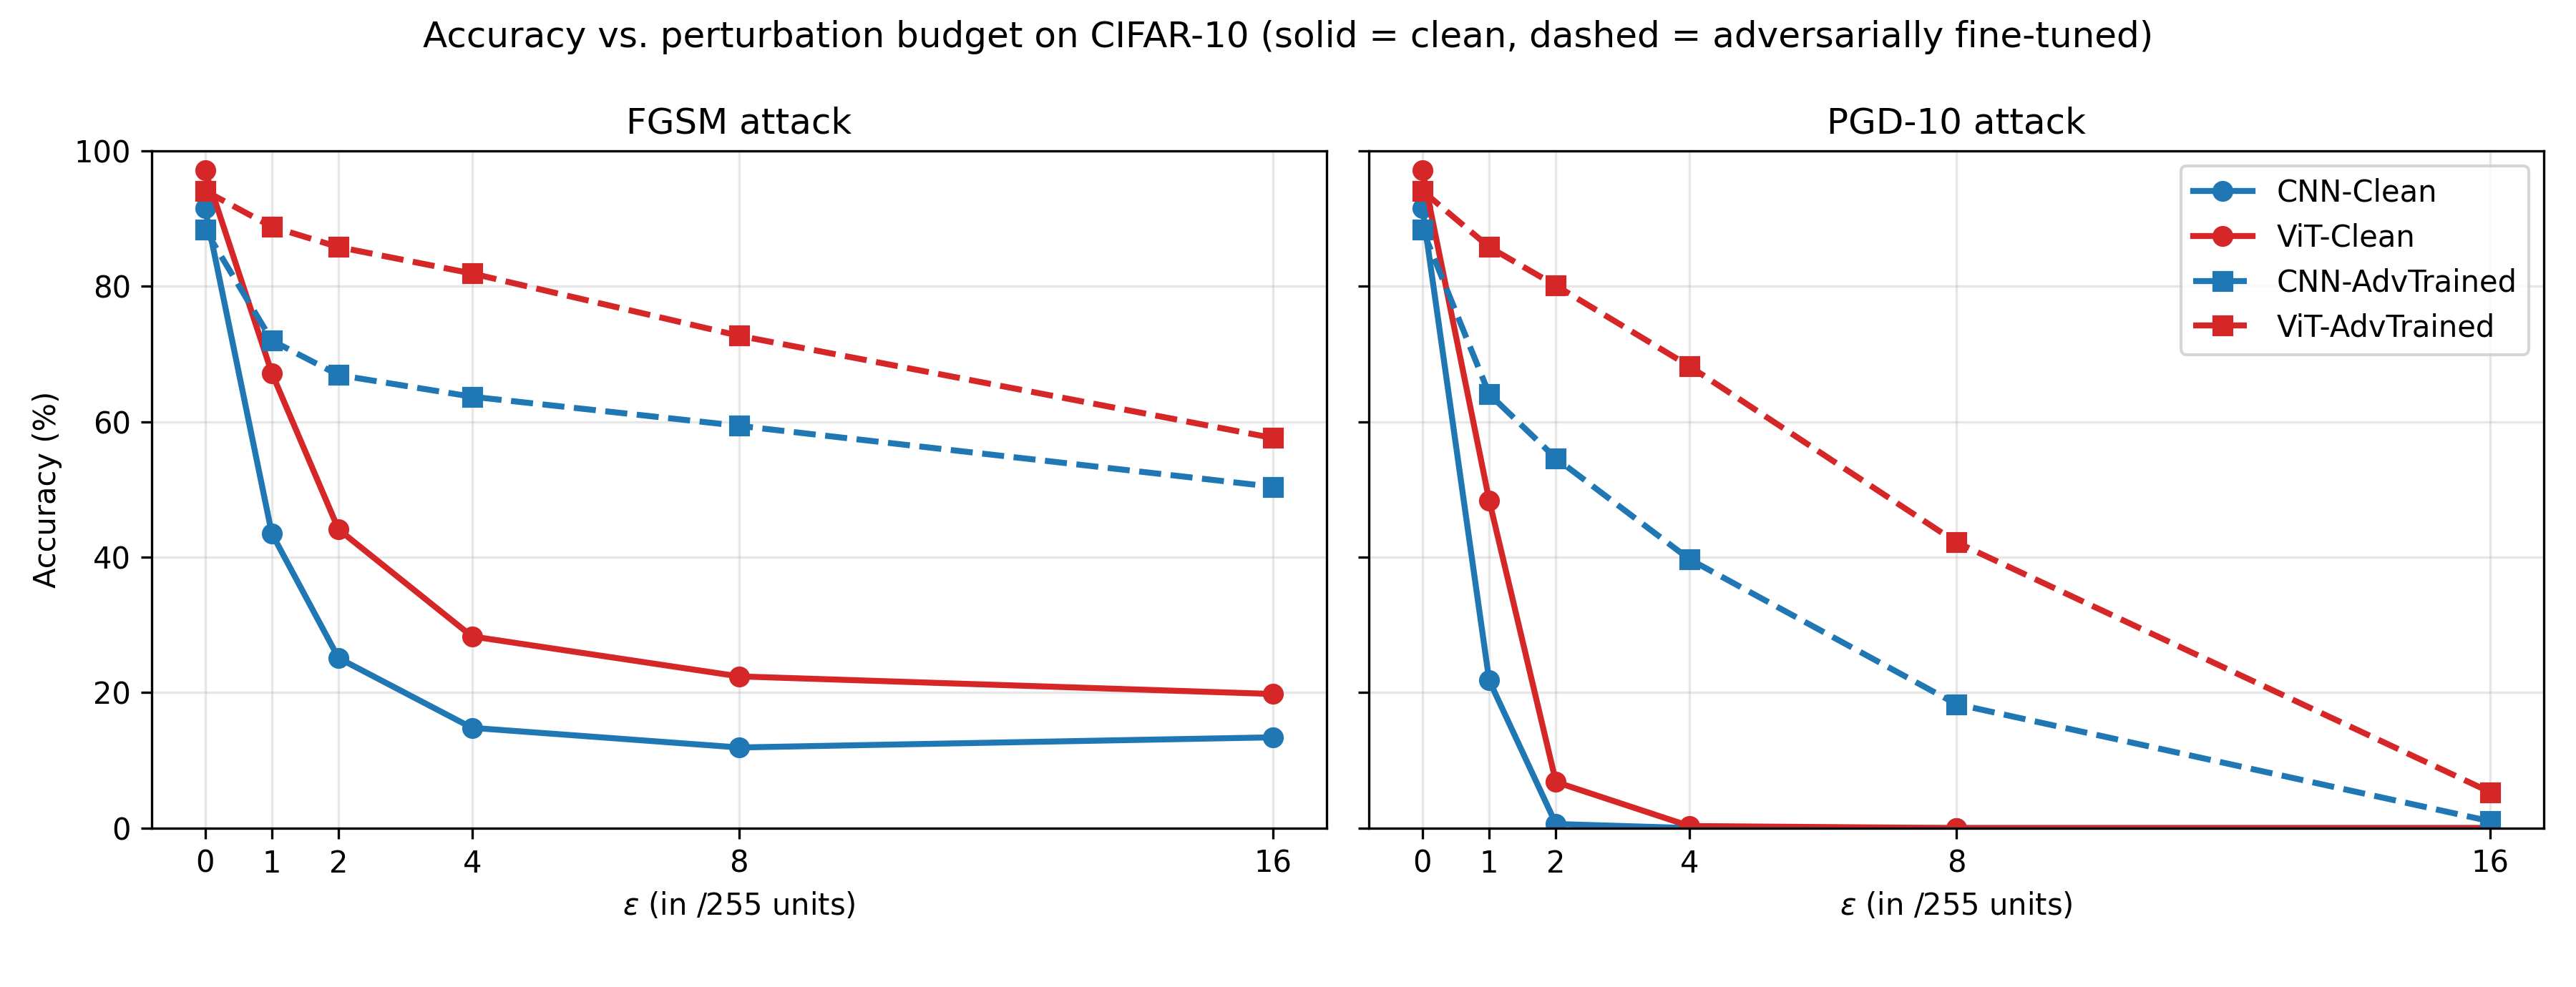
\includegraphics[width=\textwidth]{figures/acc_vs_epsilon.png}}
\caption{Accuracy versus $\epsilon$ (in units of 1/255) under FGSM
(left) and PGD-10 (right). Solid lines: clean models. Dashed lines:
adversarially fine-tuned models. Blue: CNN. Red: ViT.}
\label{fig:acc}
\end{figure}

\begin{table}[h]
\centerline{
\begin{tabular}{|l|c|c|c|}
\hline
Model & Clean & FGSM & PGD-10 \\ \hline \hline
CNN-Clean (ResNet-20)    & 91.5 & 11.9 & 0.0  \\
CNN-AdvTrained (PGD-5)   & 88.4 & 59.4 & 18.3 \\ \hline
ViT-Clean (ViT-Tiny)     & 97.1 & 22.4 & 0.0  \\
ViT-AdvTrained (PGD-5)   & 94.1 & 72.7 & 42.2 \\ \hline
\end{tabular}
}
\caption{Accuracy (\%) on 1000 test images at $\epsilon = 8/255$.}
\label{tab:main}
\end{table}

\begin{table}[h]
\centerline{
\small
\begin{tabular}{|l|l|c|c|c|c|c|c|}
\hline
Attack & Model & 0 & 1/255 & 2/255 & 4/255 & 8/255 & 16/255 \\ \hline \hline
FGSM   & CNN-Clean      & 91.5 & 43.5 & 25.1 & 14.8 & 11.9 & 13.4 \\
       & ViT-Clean      & 97.1 & 67.2 & 44.1 & 28.3 & 22.4 & 19.8 \\
       & CNN-AdvTrained & 88.4 & 72.0 & 66.9 & 63.7 & 59.4 & 50.4 \\
       & ViT-AdvTrained & 94.1 & 88.8 & 85.8 & 81.9 & 72.7 & 57.6 \\ \hline
PGD-10 & CNN-Clean      & 91.5 & 21.8 & 0.6  & 0.0  & 0.0  & 0.0  \\
       & ViT-Clean      & 97.1 & 48.4 & 6.8  & 0.3  & 0.0  & 0.0  \\
       & CNN-AdvTrained & 88.4 & 64.1 & 54.6 & 39.7 & 18.3 & 1.0  \\
       & ViT-AdvTrained & 94.1 & 85.8 & 80.1 & 68.2 & 42.2 & 5.3  \\ \hline
\end{tabular}
}
\caption{Accuracy (\%) for every model, attack and $\epsilon$
($N = 1000$).}
\label{tab:full}
\end{table}

Without defence, both networks fail quickly. Under PGD-10 the CNN falls
to 21.8\% at $\epsilon = 1/255$ and 0.6\% at $2/255$, and the ViT to
48.4\% and 6.8\%. Both are at about 0\% from $4/255$. The ViT keeps more
accuracy at small budgets, and under FGSM at $8/255$ it keeps 22.4\%
against 11.9\% for the CNN.

After adversarial fine-tuning, the PGD-10 curves of both models move up at
every budget up to $8/255$. The ViT is ahead of the CNN by 21.7, 25.5,
28.5 and 23.9 points at $\epsilon = 1, 2, 4$ and $8/255$, and by 4.3
points at $16/255$, where both models are close to 0\%. At twice the
training budget neither model is robust.

\subsection{Cost of adversarial training}

Figure~\ref{fig:tradeoff} compares each model before and after
fine-tuning.

\begin{figure}[t]
\centerline{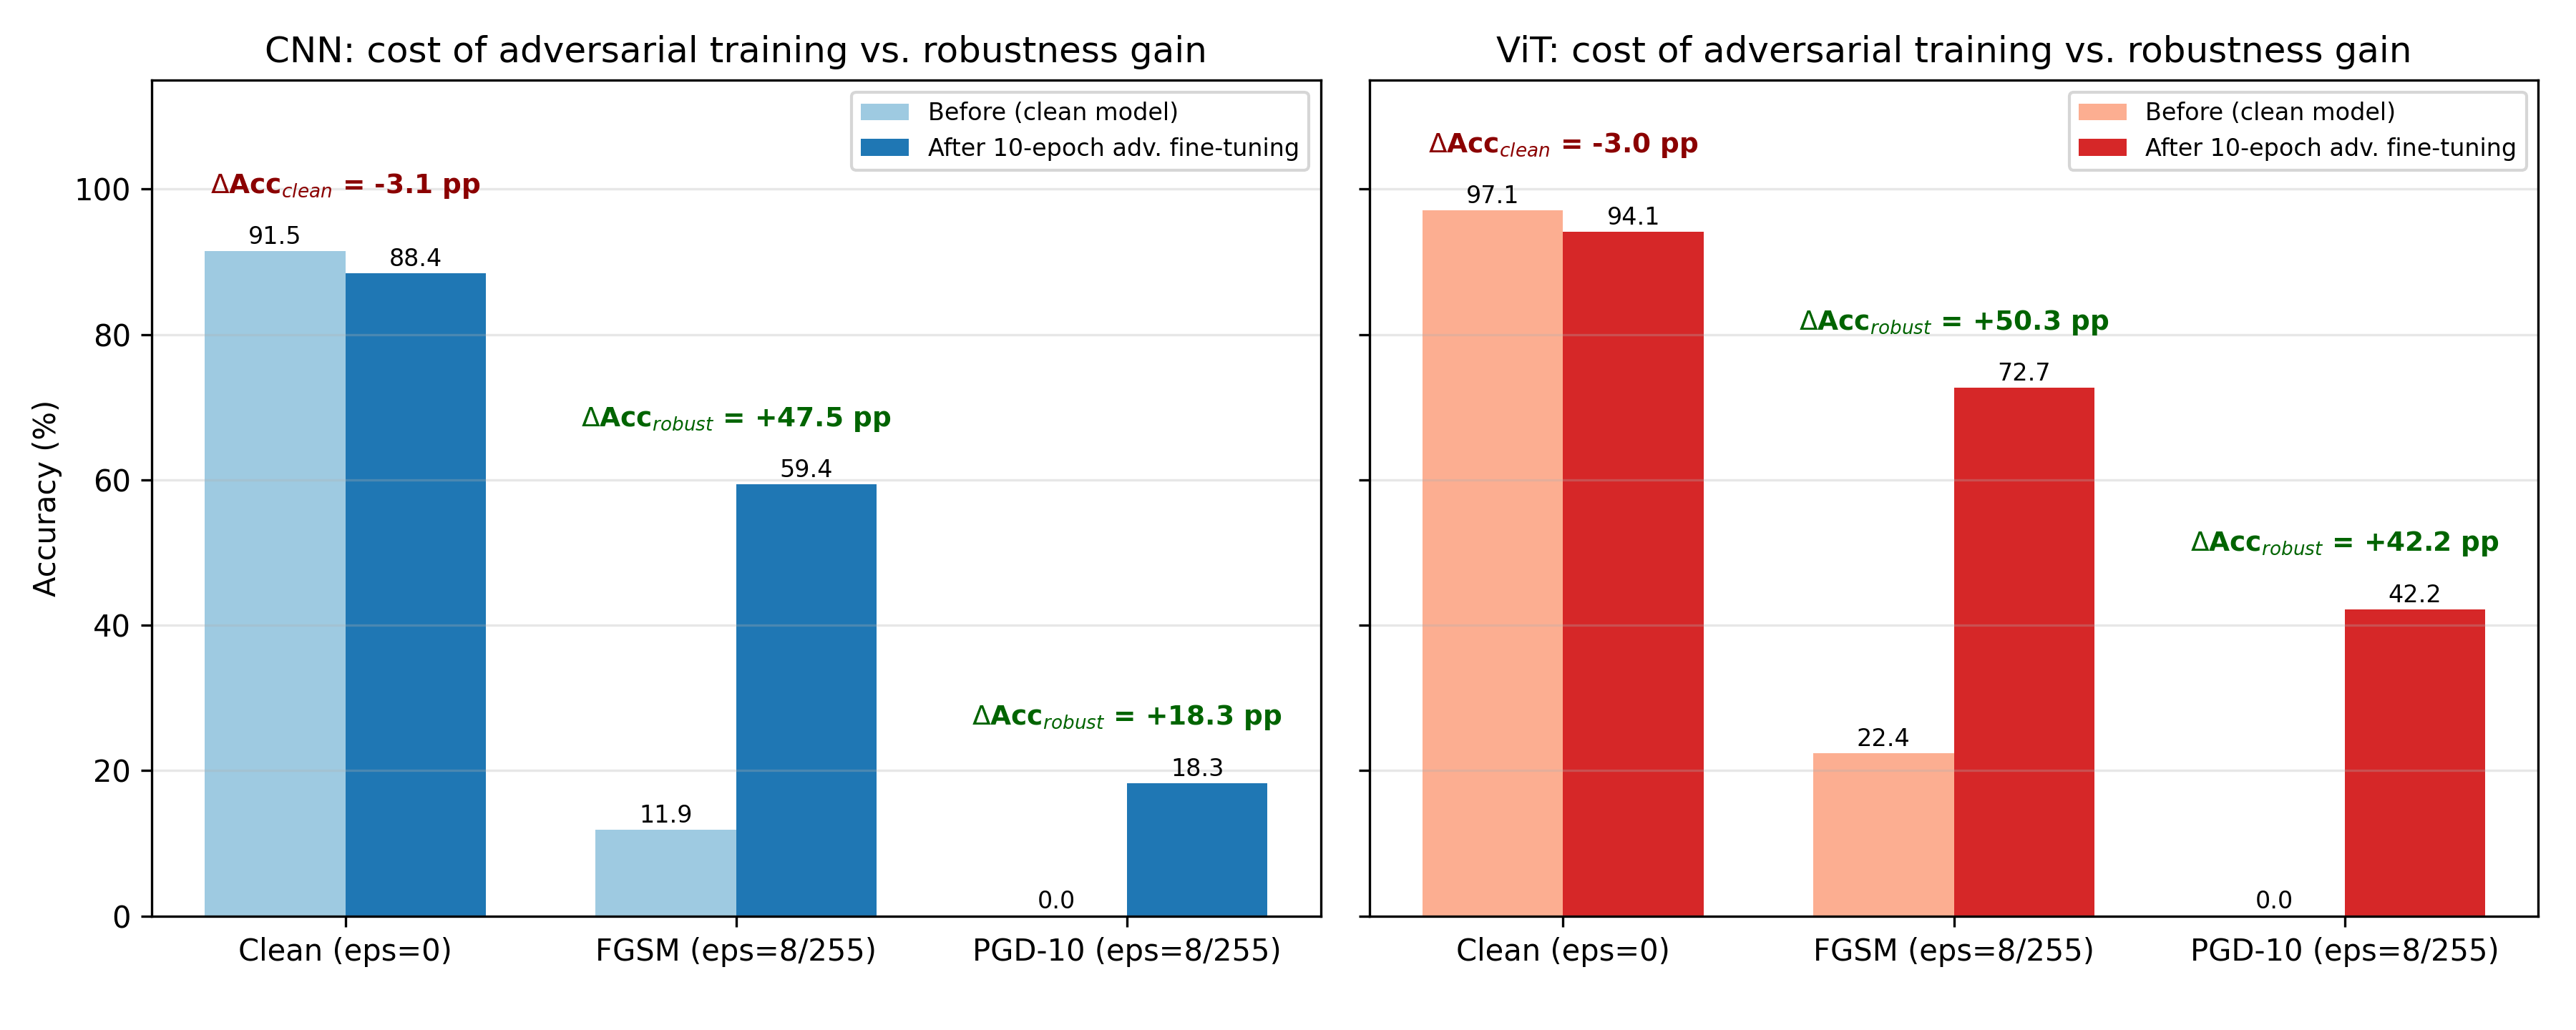
\includegraphics[width=\textwidth]{figures/clean_vs_robust_tradeoff.png}}
\caption{Change in clean, FGSM and PGD-10 accuracy ($\epsilon = 8/255$)
caused by 10 epochs of adversarial fine-tuning. Left: CNN. Right: ViT.}
\label{fig:tradeoff}
\end{figure}

Clean accuracy falls by 3.1 points for the CNN (91.5\% to 88.4\%) and by
3.0 points for the ViT (97.1\% to 94.1\%). The two costs are practically
equal. In return, PGD-10 accuracy at $8/255$ rises by 18.3 points for the
CNN and by 42.2 points for the ViT. FGSM accuracy rises by 47.5 and 50.3
points. The ViT gets more robustness for the same loss of clean accuracy.

\subsection{Why single-step training was not enough}

Our first ViT run used RS-FGSM instead of PGD-5 for adversarial training,
because it is about 2.5 times faster (30.1 min instead of 74.7 min on the
T4). Table~\ref{tab:rs} compares the two ViT models.

\begin{table}[h]
\centerline{
\begin{tabular}{|l|l|c|c|c|c|c|}
\hline
Training attack & Test attack & 1/255 & 2/255 & 4/255 & 8/255 & 16/255 \\ \hline \hline
RS-FGSM & FGSM   & 81.2 & 68.4 & 67.7 & 79.8 & 52.6 \\
        & PGD-10 & 75.7 & 40.4 & 11.9 & 4.9  & 0.0  \\ \hline
PGD-5   & FGSM   & 88.8 & 85.8 & 81.9 & 72.7 & 57.6 \\
        & PGD-10 & 85.8 & 80.1 & 68.2 & 42.2 & 5.3  \\ \hline
\end{tabular}
}
\caption{ViT-AdvTrained accuracy (\%) for two training attacks.}
\label{tab:rs}
\end{table}

The RS-FGSM model scores 79.8\% under FGSM at $8/255$ but only 4.9\%
under PGD-10. Its FGSM accuracy also rises from 67.7\% at $4/255$ to
79.8\% at $8/255$, a peak exactly at the training budget. A model that is
really robust should not become more accurate when the attack gets
stronger. This pattern is typical of catastrophic overfitting
\cite{Wong:20}. Training with PGD-5 removes the peak and raises PGD-10
accuracy at $8/255$ from 4.9\% to 42.2\%, which is consistent with that
explanation. The two runs also differ slightly in ViT-Clean (97.4\% and
97.1\%, because the clean fine-tune was repeated), so this is supporting
evidence and not an isolated test. The practical lesson is to judge
robustness with PGD, not with FGSM alone. The CNN-versus-ViT comparison in
this report uses PGD-5 for both models.

\subsection{Transferability}

Figure~\ref{fig:transfer} and Table~\ref{tab:transfer} show the accuracy
of each target model on PGD-10 examples crafted on each source model.

\begin{figure}[t]
\centerline{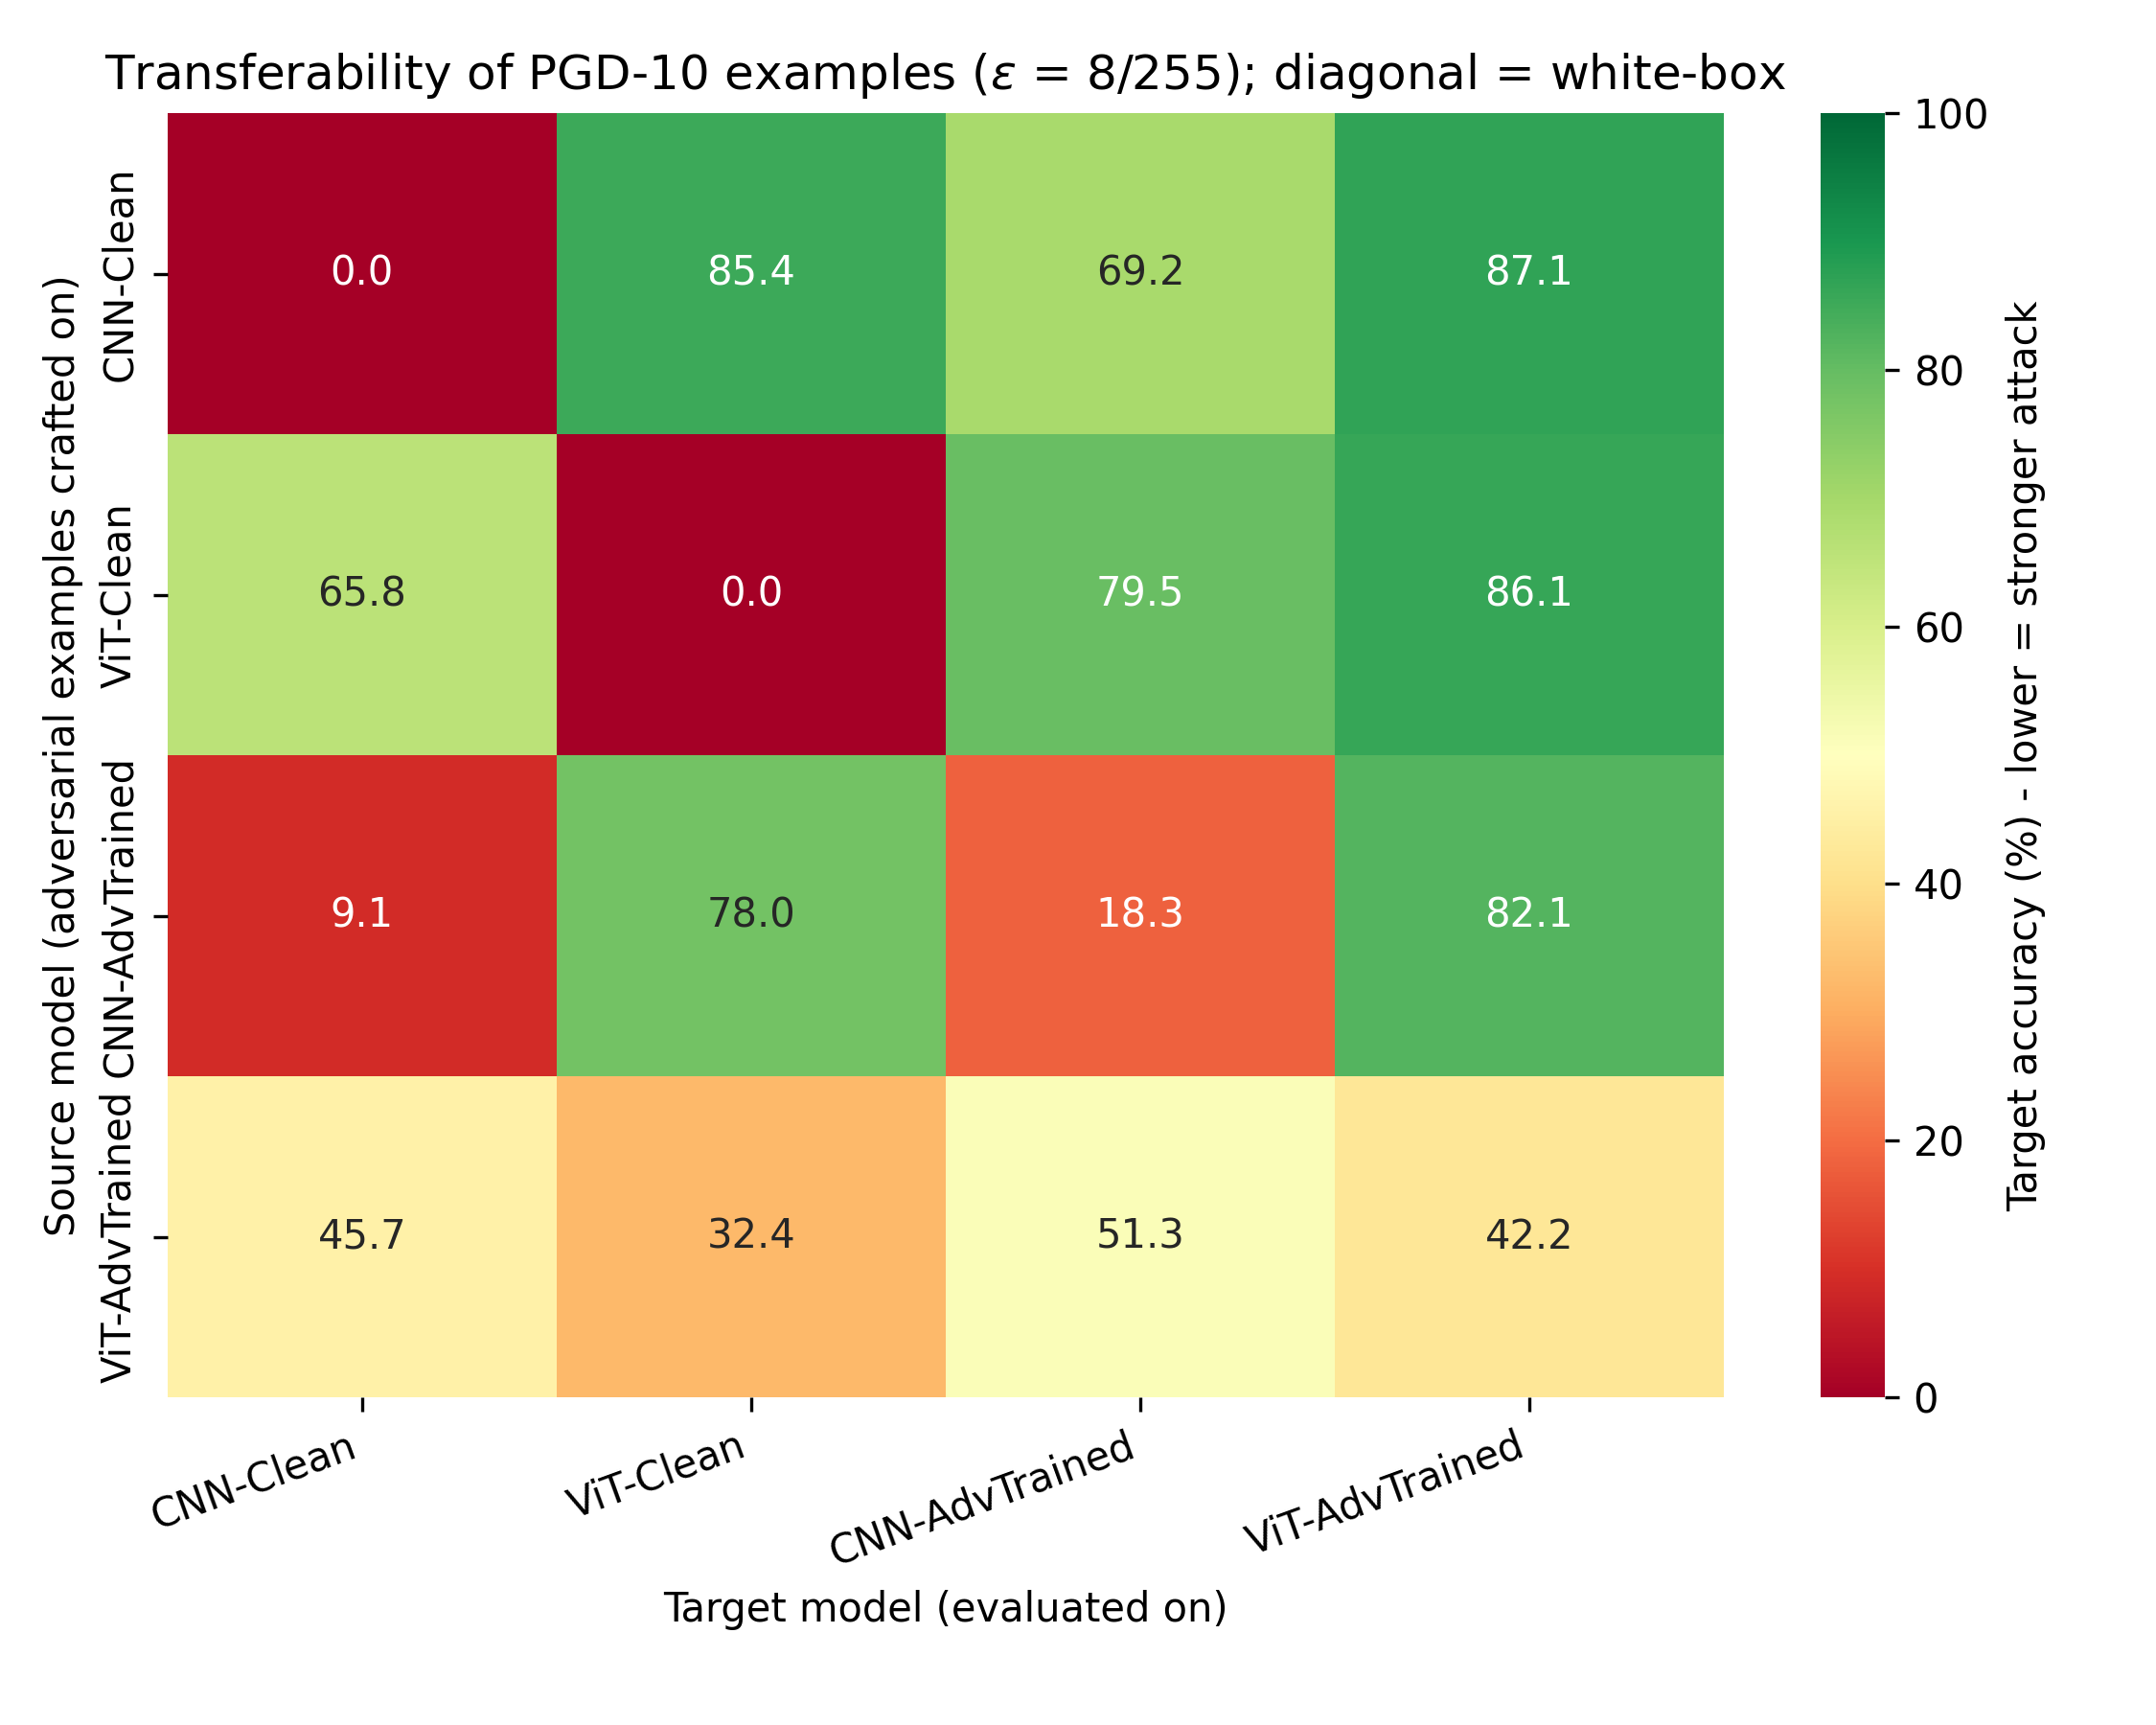
\includegraphics[width=0.62\textwidth]{figures/transferability_heatmap.png}}
\caption{Transferability of PGD-10 examples ($\epsilon = 8/255$).
Rows: source model. Columns: target model. Values: target accuracy (\%).
The diagonal is the white-box case.}
\label{fig:transfer}
\end{figure}

\begin{table}[h]
\centerline{
\begin{tabular}{|l|c|c|c|c|}
\hline
Source $\backslash$ Target & CNN-Clean & ViT-Clean & CNN-Adv & ViT-Adv \\ \hline \hline
CNN-Clean & 0.0  & 85.4 & 69.2 & 87.1 \\
ViT-Clean & 65.8 & 0.0  & 79.5 & 86.1 \\
CNN-Adv   & 9.1  & 78.0 & 18.3 & 82.1 \\
ViT-Adv   & 45.7 & 32.4 & 51.3 & 42.2 \\ \hline
\end{tabular}
}
\caption{Target accuracy (\%) under transferred PGD-10 examples,
$\epsilon = 8/255$.}
\label{tab:transfer}
\end{table}

White-box attacks are far stronger than transferred ones. Examples from
CNN-Clean leave ViT-Clean at 85.4\%, and examples from ViT-Clean leave
CNN-Clean at 65.8\%. Compared with the clean accuracy of each target, this
is a drop of 11.7 points (CNN to ViT) and 25.7 points (ViT to CNN), so
perturbations transfer more easily from the ViT to the CNN than the other
way round. Adversarially trained targets resist transfer from clean
sources better (CNN-Clean to CNN-AdvTrained 69.2\%, ViT-Clean to
ViT-AdvTrained 86.1\%). Models from the same family transfer strongly:
examples from CNN-AdvTrained leave CNN-Clean at 9.1\%, and examples from
ViT-AdvTrained leave ViT-Clean at 32.4\%, which is expected since each
adversarial model was fine-tuned from its clean version. Finally,
transferred examples leave ViT-AdvTrained at 82 to 87\%, while a
white-box attack leaves it at 42.2\%. A transfer (black-box) test alone
would therefore overstate its robustness.

\subsection{Qualitative examples}

Figure~\ref{fig:grid} shows four test images, the magnified perturbation
$(x_{\mathrm{adv}} - x + \epsilon)/(2\epsilon)$ and the adversarial image
at $\epsilon = 8/255$, crafted on CNN-Clean with PGD-10. The adversarial
images look the same as the originals. CNN-Clean misclassifies all four
(frog as dog, truck as automobile, dog as bird, ship as frog), while the
other three models classify all four correctly. Four images are only an
illustration. The quantitative evidence is in the tables above.

\begin{figure}[t]
\centerline{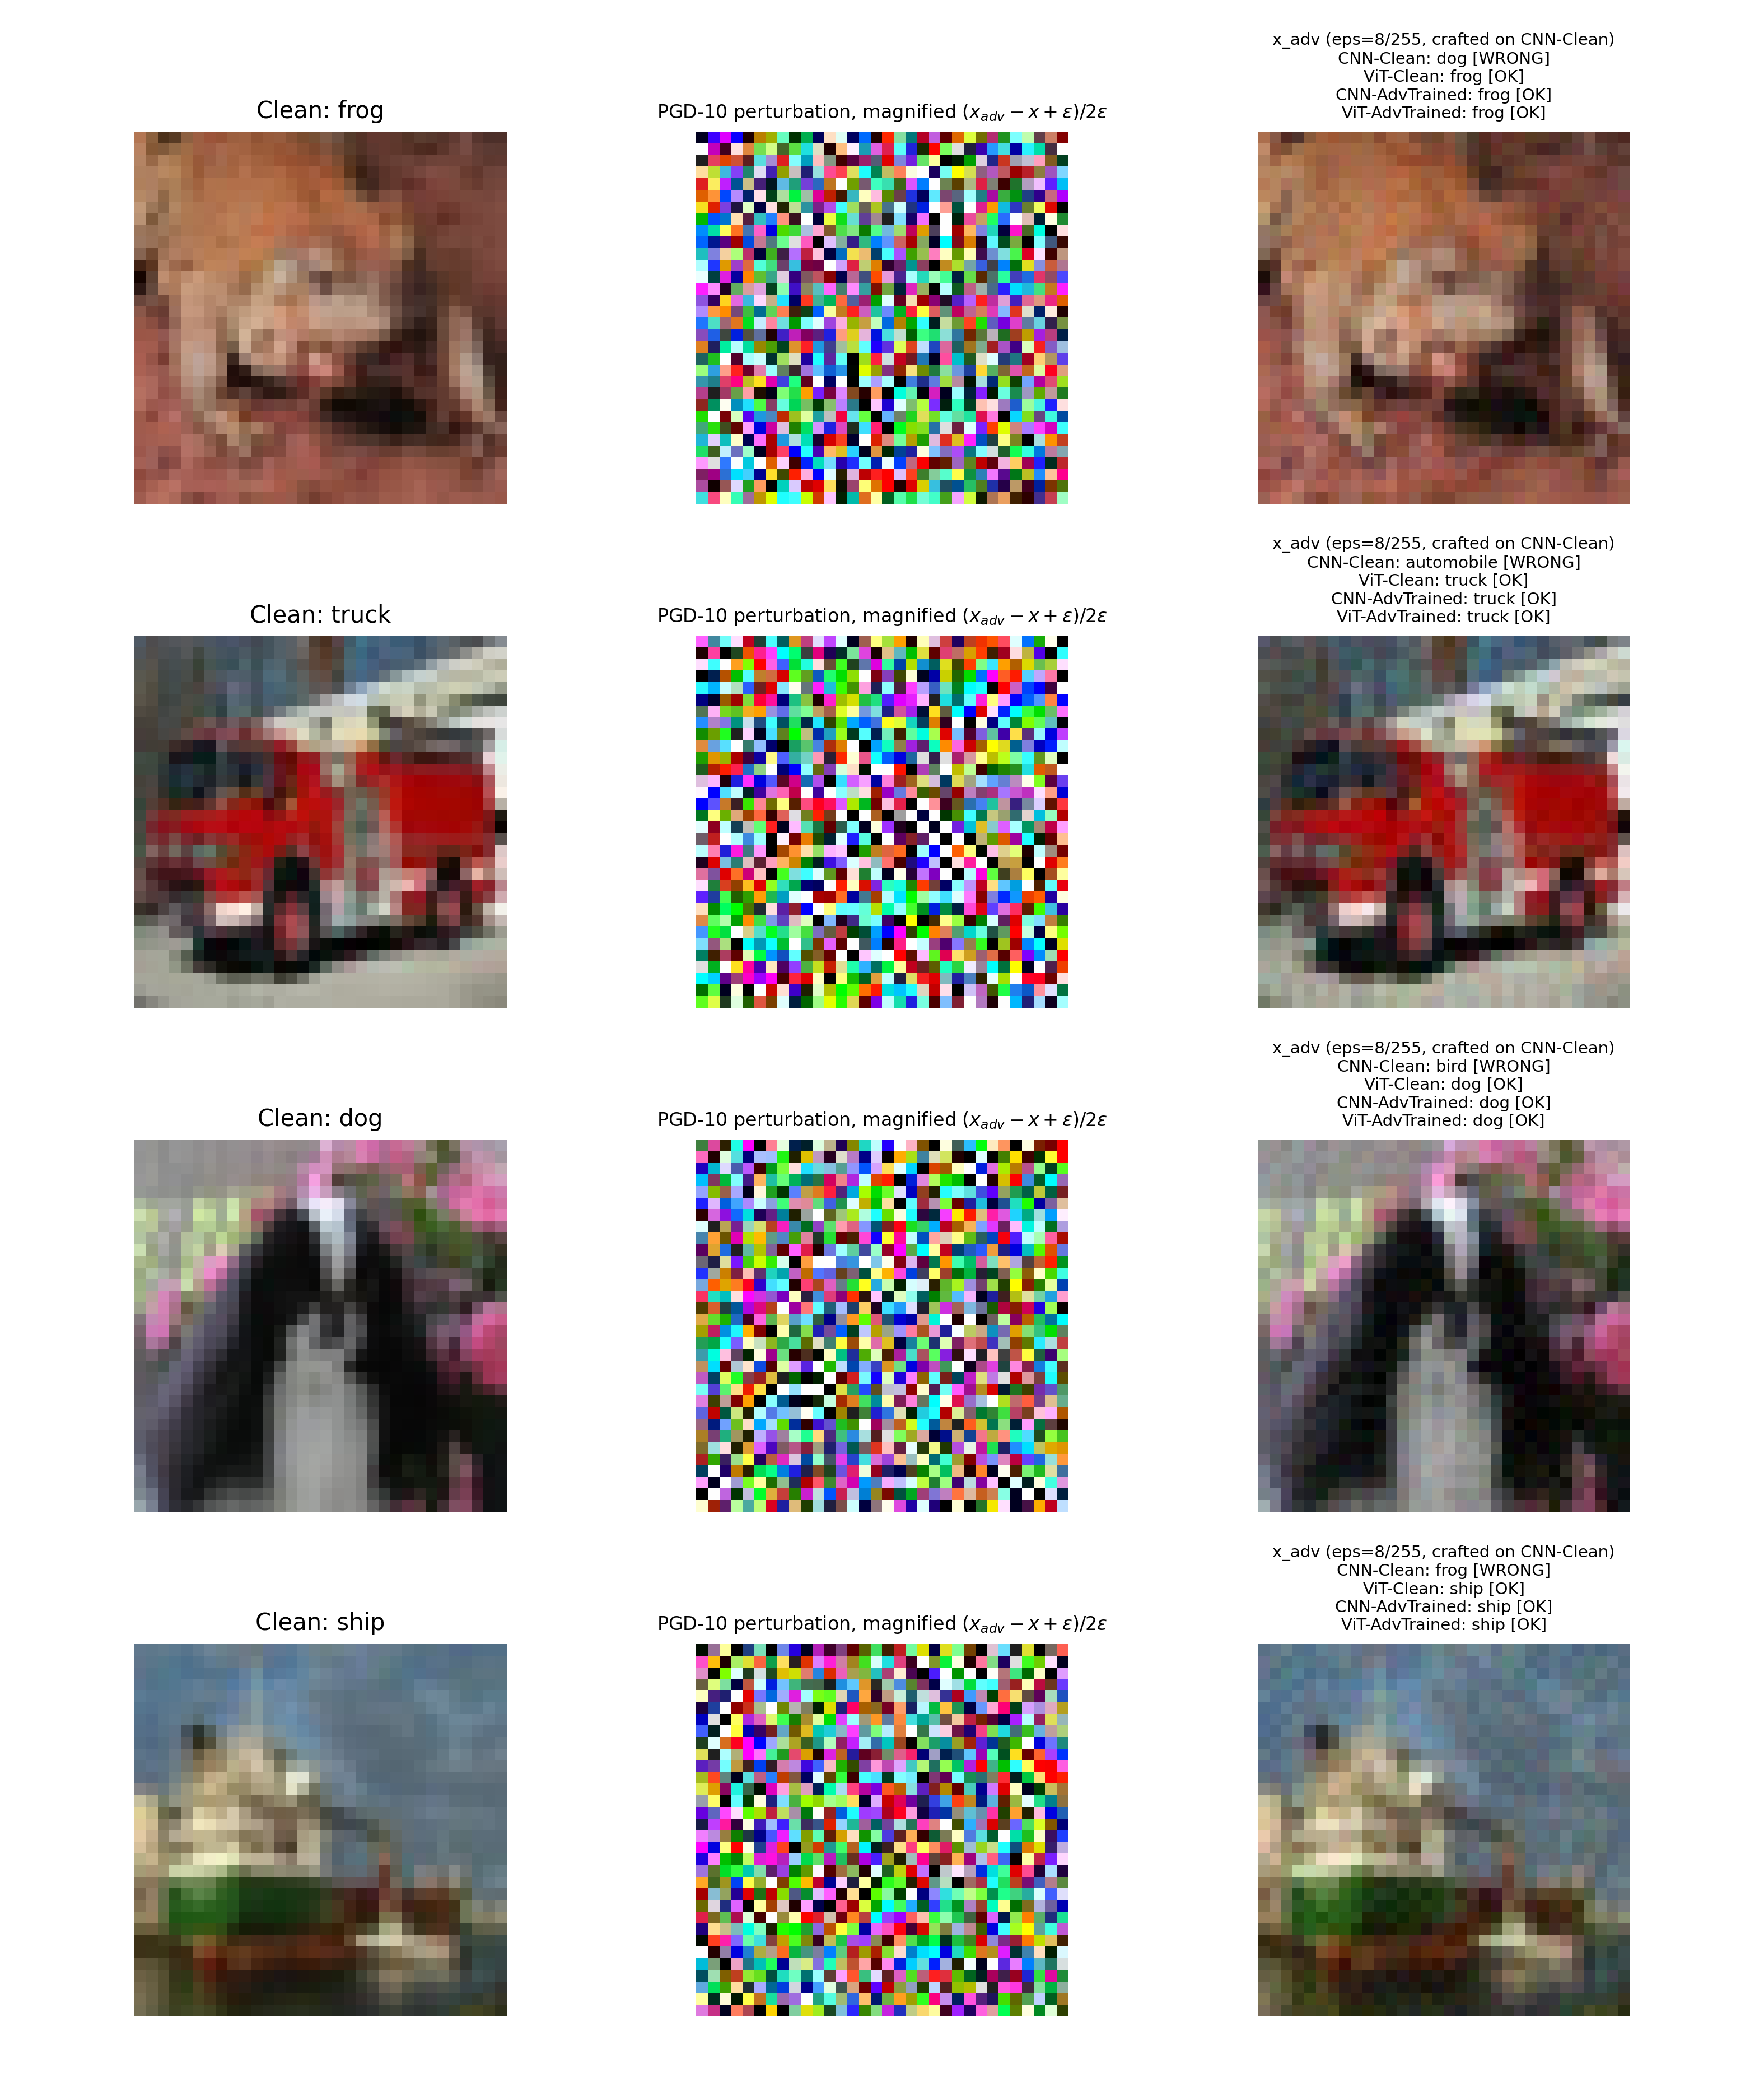
\includegraphics[width=0.58\textwidth]{figures/adversarial_examples_grid.png}}
\caption{Clean image (left), magnified PGD-10 perturbation (middle) and
adversarial image at $\epsilon = 8/255$ (right) with the predictions of
the four models.}
\label{fig:grid}
\end{figure}

\section{Discussion}

\textbf{RQ1: robustness across architectures.} Under the same training
recipe, the adversarially trained ViT is more robust than the adversarially
trained CNN at every tested $\epsilon$ from $1/255$ to $16/255$ (Table~\ref{tab:full}).
The clean ViT also keeps more accuracy than the clean CNN at small budgets
(PGD-10 at $1/255$: 48.4\% against 21.8\%), but it also starts from a higher
clean accuracy (97.1\% against 91.5\%). Moreover, this comparison involves two specific networks, and
architecture is not the only difference. ViT-Tiny has about 20 times more
parameters than ResNet-20, is pretrained on ImageNet and sees $224 \times
224$ inputs. Model capacity is known to matter for adversarial training
\cite{Madry:18}. These results do not show that self-attention itself
causes the extra robustness.

\textbf{RQ2: cost of adversarial training.} Ten epochs of PGD-5 fine-tuning
cost about 3 points of clean accuracy for both models. The size of the
robustness gain depends on the model and the attack, from +18.3 to +42.2
points under PGD-10 at $8/255$.

\textbf{Limitations.}
\begin{itemize}
\item \emph{Sample size and seeds.} Results use 1000 test images and one
training run per model with seed 42, so there is no estimate of
variation across training seeds.
\item \emph{Attack strength.} PGD-10 accuracy is an upper bound on true
robust accuracy. Stronger attacks (more steps, restarts, AutoAttack)
would lower the numbers, and no certified robustness is claimed.
\item \emph{Robust generalisation gap.} For both models, the adversarial
accuracy on training batches in the last epoch (CNN 31.8\%, ViT 59.1\%)
is higher than the PGD-10 test accuracy at $8/255$ (18.3\% and 42.2\%).
The attacks and data augmentation differ between the two measurements, so
the gap is only indicative.
\item \emph{Short fine-tuning.} Only 10 epochs from pretrained weights
were used, which keeps the run on a free GPU but is shorter than
training robust models from scratch.
\item \emph{Two Colab sessions.} The CNN results come from the first
session. The ViT results come from a second session that re-ran the clean
ViT fine-tune, because that checkpoint had not been saved. The CNN
checkpoint is identical between sessions.
\end{itemize}

\section{Conclusion}

We implemented FGSM and PGD from scratch and measured the robustness of a
ResNet-20 and a ViT-Tiny on CIFAR-10 before and after 10 epochs of PGD-5
adversarial fine-tuning. Undefended models are fooled almost completely by
a PGD perturbation of $8/255$. Adversarial fine-tuning costs about 3
points of clean accuracy for both models and raises PGD-10 accuracy at
$8/255$ to 18.3\% (CNN) and 42.2\% (ViT). The ViT is more robust than the
CNN at every tested budget, though model size and pretraining differ
between them. A ViT trained with the cheaper RS-FGSM attack looked robust
under FGSM but was not robust under PGD, so single-step attacks should not
be the only evaluation. Future work includes repeating the runs with
several seeds, testing stronger attacks such as AutoAttack, and comparing
models of similar size and pretraining.

\begin{thebibliography}{99}

\bibitem{Szegedy:14}
C. Szegedy, W. Zaremba, I. Sutskever, J. Bruna, D. Erhan, I. Goodfellow,
R. Fergus, "Intriguing properties of neural networks",
{\em Intl. Conf. on Learning Representations (ICLR)}, 2014.

\bibitem{Goodfellow:15}
I. J. Goodfellow, J. Shlens, C. Szegedy, "Explaining and Harnessing
Adversarial Examples", {\em Intl. Conf. on Learning Representations
(ICLR)}, 2015. https://arxiv.org/abs/1412.6572

\bibitem{Madry:18}
A. Madry, A. Makelov, L. Schmidt, D. Tsipras, A. Vladu, "Towards Deep
Learning Models Resistant to Adversarial Attacks", {\em Intl. Conf. on
Learning Representations (ICLR)}, 2018. https://arxiv.org/abs/1706.06083

\bibitem{Wong:20}
E. Wong, L. Rice, J. Z. Kolter, "Fast is better than free: Revisiting
adversarial training", {\em Intl. Conf. on Learning Representations
(ICLR)}, 2020. https://arxiv.org/abs/2001.03994

\bibitem{He:16}
K. He, X. Zhang, S. Ren, J. Sun, "Deep Residual Learning for Image
Recognition", {\em IEEE Conf. on Computer Vision and Pattern Recognition
(CVPR)}, 2016.

\bibitem{Dosovitskiy:21}
A. Dosovitskiy et al., "An Image is Worth 16x16 Words: Transformers for
Image Recognition at Scale", {\em Intl. Conf. on Learning Representations
(ICLR)}, 2021.

\bibitem{Krizhevsky:09}
A. Krizhevsky, "Learning Multiple Layers of Features from Tiny Images",
Technical Report, University of Toronto, 2009.

\bibitem{Chenyaofo}
Y. Chen, "PyTorch CIFAR models: pretrained ResNet, MobileNet and other
models for CIFAR-10/100", GitHub repository
\texttt{chenyaofo/pytorch-cifar-models}.

\bibitem{Wightman:19}
R. Wightman, "PyTorch Image Models (timm)", GitHub repository
\texttt{huggingface/pytorch-image-models}, 2019.

\bibitem{Loshchilov:19}
I. Loshchilov, F. Hutter, "Decoupled Weight Decay Regularization",
{\em Intl. Conf. on Learning Representations (ICLR)}, 2019.

\bibitem{Micikevicius:18}
P. Micikevicius et al., "Mixed Precision Training", {\em Intl. Conf. on
Learning Representations (ICLR)}, 2018.

\bibitem{Paszke:19}
A. Paszke et al., "PyTorch: An Imperative Style, High-Performance Deep
Learning Library", {\em Advances in Neural Information Processing Systems
(NeurIPS)}, 2019.

\end{thebibliography}

\end{document}
